%
% A header that lets you compile a chapter by itself, or inside a larger document.
% Adapted from http://stackoverflow.com/questions/3655454/conditional-import-in-latex
%
%
%Use \inbpdocument and \outbpdocument in your individual files, in place of \begin{document} and \end{document}. In your main file, put in a \def \ismaindoc {} before including or importing anything.
%
% David Duvenaud
% June 2011
% 
% ======================================
%
%


\ifx\ismaindoc\undefined
	\newcommand{\inbpdocument}{
		\def \ismaindoc {}
		% Use this header if we are compiling by ourselves.
		\documentclass[a4paper,11pt,authoryear,index]{common/PhDThesisPSnPDF}
		
%\usepackage{draftwatermark}
%\SetWatermarkLightness{0.95}

% ******************************************************************************
% ****************************** Custom Margin *********************************

% Add `custommargin' in the document class options to use this section
% Set {innerside margin / outerside margin / topmargin / bottom margin}  and
% other page dimensions

\ifsetMargin
\else
    \RequirePackage[left=37mm,right=30mm,top=35mm,bottom=30mm]{geometry}
    \setFancyHdr % To apply fancy header after geometry package is loaded
\fi


%\chead{Unfinished draft}
%\cfoot{\texttt{Unfinished draft - compiled on \today{} at \currenttime}}

% *****************************************************************************
% ******************* Fonts (like different typewriter fonts etc.)*************

% Add `customfont' in the document class option to use this section

\ifsetFont
\else
    % Set your custom font here and use `customfont' in options. Leave empty to
    % load computer modern font (default LaTeX font).  

    \RequirePackage{libertine} 
\fi

% *****************************************************************************
% *************************** Bibliography  and References ********************

%\usepackage{cleveref} %Referencing without need to explicitly state fig /table

% Add `custombib' in the document class option to use this section
\ifsetBib % True, Bibliography option is chosen in class options
\else % If custom bibliography style chosen then load bibstyle here

   \RequirePackage[square, sort, numbers, authoryear]{natbib} % CustomBib

% If you would like to use biblatex for your reference management, as opposed to the default `natbibpackage` pass the option `custombib` in the document class. Comment out the previous line to make sure you don't load the natbib package. Uncomment the following lines and specify the location of references.bib file

% \RequirePackage[backend=biber, style=numeric-comp, citestyle=numeric, sorting=nty, natbib=true]{biblatex}
% \bibliography{References/references} %Location of references.bib only for biblatex

\fi


% changes the default name `Bibliography` -> `References'
\renewcommand{\bibname}{References}


% *****************************************************************************
% *************** Changing the Visual Style of Chapter Headings ***************
% Uncomment the section below. Requires titlesec package.

%\RequirePackage{titlesec}
%\newcommand{\PreContentTitleFormat}{\titleformat{\chapter}[display]{\scshape\Large}
%{\Large\filleft{\chaptertitlename} \Huge\thechapter}
%{1ex}{}
%[\vspace{1ex}\titlerule]}
%\newcommand{\ContentTitleFormat}{\titleformat{\chapter}[display]{\scshape\huge}
%{\Large\filleft{\chaptertitlename} \Huge\thechapter}{1ex}
%{\titlerule\vspace{1ex}\filright}
%[\vspace{1ex}\titlerule]}
%\newcommand{\PostContentTitleFormat}{\PreContentTitleFormat}
%\PreContentTitleFormat


% *****************************************************************************
% **************************** Custom Packages ********************************
% *****************************************************************************


% ************************* Algorithms and Pseudocode **************************

%\usepackage{algpseudocode} 


% ********************Captions and Hyperreferencing / URL **********************

% Captions: This makes captions of figures use a boldfaced small font. 
%\RequirePackage[small,bf]{caption}

\RequirePackage[labelsep=space,tableposition=top]{caption} 
%\renewcommand{\figurename}{Figure} %to support older versions of captions.sty
\captionsetup{belowskip=12pt,aboveskip=4pt}

% ************************ Formatting / Footnote *******************************

%\usepackage[perpage]{footmisc} %Range of footnote options 


% ****************************** Line Numbers **********************************

%\RequirePackage{lineno}
%\linenumbers

% ************************** Graphics and figures *****************************

%\usepackage{rotating}
%\usepackage{wrapfig}
%\usepackage{float}
\usepackage{subfig} %note: subfig must be included after the `caption` package. 


% ********************************* Table **************************************

%\usepackage{longtable}
%\usepackage{multicol}
%\usepackage{multirow}
%\usepackage{tabularx}


% ***************************** Math and SI Units ******************************

\usepackage{amsfonts}
\usepackage{amsmath}
\usepackage{amssymb}
%\usepackage{siunitx} % use this package module for SI units


% ******************************************************************************
% ************************* User Defined Commands ******************************
% ******************************************************************************

% *********** To change the name of Table of Contents / LOF and LOT ************

%\renewcommand{\contentsname}{My Table of Contents}
%\renewcommand{\listfigurename}{List of figures}
%\renewcommand{\listtablename}{List of tables}


% ********************** TOC depth and numbering depth *************************

\setcounter{secnumdepth}{2}
\setcounter{tocdepth}{2}

% ******************************* Nomenclature *********************************

% To change the name of the Nomenclature section, uncomment the following line

%\renewcommand{\nomname}{Symbols}


% ********************************* Appendix ***********************************

% The default value of both \appendixtocname and \appendixpagename is `Appendices'. These names can all be changed via: 

%\renewcommand{\appendixtocname}{List of appendices}
%\renewcommand{\appendixname}{Appndx}

		% All my custom preamble stuff.  Shouldn't overlap with anything in official-preamble


% Paths to figure and table directories.
\newcommand{\symmetryfigsdir}{figures/symmetries}
\newcommand{\topologyfiguresdir}{figures/topology}
\newcommand{\infinitefiguresdir}{figures/infinite}
\newcommand{\grammarfiguresdir}{figures/grammar}
\newcommand{\introfigsdir}{figures/intro}
\newcommand{\gplvmfiguresdir}{figures/gplvm}
\newcommand{\warpedfiguresdir}{figures/warped-mixtures}
\newcommand{\deeplimitsfiguresdir}{figures/deep-limits}
\newcommand{\quadraturefigsdir}{figures/quadrature}
\newcommand{\additivefigsdir}{figures/additive}
\newcommand{\decompfigsdir}{figures/decomp}
\newcommand{\examplefigsdir}{figures/worked-example}


\usepackage{bm}  % for warped mixtures - is this necessary?
\usepackage{booktabs}
\usepackage{tabularx}
\usepackage{multirow}
\usepackage{datetime}
\renewcommand{\tabularxcolumn}[1]{>{\arraybackslash}m{#1}}
\usepackage{relsize}
\usepackage{graphicx}
\usepackage{amsmath,amssymb,textcomp}
\usepackage{nicefrac}
\usepackage{amsthm}
\usepackage{tikz}
\usetikzlibrary{arrows}
\usetikzlibrary{calc}
\usepackage{nth}
\usepackage{rotating}
\usepackage{array}
\usepackage{fp}
\usepackage[hyperpageref]{backref}
\def\foo{\hspace{\fill}\mbox{}\linebreak[0]\hspace*{\fill}}
\renewcommand*{\backref}[1]{}
\renewcommand*{\backrefalt}[4]{%
\ifcase #1 %
%
\or
\foo(page #2)%
\else
\foo(pages #2)%
\fi
}

\usepackage{cleveref}
\crefname{equation}{equation}{equations}


%% For submission, make all render blank.
%%%%%%%%%%%%%%%%%%%%%%%%%%%%%%%%%%%%%%%%%%%%%%%%%%%%%%%%%%
%%%% EDITING HELPER FUNCTIONS  %%%%%%%%%%%%%%%%%%%%%%%%%%%
%%%%%%%%%%%%%%%%%%%%%%%%%%%%%%%%%%%%%%%%%%%%%%%%%%%%%%%%%%

%% NA: needs attention (rough writing whose correctness needs to be verified)
%% TBD: instructions for how to fix a gap ("Describe the propagation by ...")
%% PROBLEM: bug or missing crucial bit 

%% use \fXXX versions of these macros to put additional explanation into a footnote.  
%% The idea is that we don't want to interrupt the flow of the paper or make it 
%% impossible to read because there are a bunch of comments.

%% NA's (and TBDs, those less crucially) should be written so 
%% that they flow with the text.

\definecolor{WowColor}{rgb}{.75,0,.75}
\definecolor{SubtleColor}{rgb}{0,0,.50}

% inline
\newcommand{\NA}[1]{\textcolor{SubtleColor}{ {\tiny \bf ($\star$)} #1}}
\newcommand{\LATER}[1]{\textcolor{SubtleColor}{ {\tiny \bf ($\dagger$)} #1}}
\newcommand{\TBD}[1]{\textcolor{SubtleColor}{ {\tiny \bf (!)} #1}}
\newcommand{\PROBLEM}[1]{\textcolor{WowColor}{ {\bf (!!)} {\bf #1}}}

% as margin notes

\newcounter{margincounter}
\newcommand{\displaycounter}{{\arabic{margincounter}}}
\newcommand{\incdisplaycounter}{{\stepcounter{margincounter}\arabic{margincounter}}}

\newcommand{\fTBD}[1]{\textcolor{SubtleColor}{$\,^{(\incdisplaycounter)}$}\marginpar{\tiny\textcolor{SubtleColor}{ {\tiny $(\displaycounter)$} #1}}}

\newcommand{\fPROBLEM}[1]{\textcolor{WowColor}{$\,^{((\incdisplaycounter))}$}\marginpar{\tiny\textcolor{WowColor}{ {\bf $\mathbf{((\displaycounter))}$} {\bf #1}}}}

\newcommand{\fLATER}[1]{\textcolor{SubtleColor}{$\,^{(\incdisplaycounter\dagger)}$}\marginpar{\tiny\textcolor{SubtleColor}{ {\tiny $(\displaycounter\dagger)$} #1}}}

%\renewcommand{\LATER}[1]{}
%\renewcommand{\fLATER}[1]{}
%\renewcommand{\TBD}[1]{}
%\renewcommand{\fTBD}[1]{}
%\renewcommand{\PROBLEM}[1]{}
%\renewcommand{\fPROBLEM}[1]{}
%\renewcommand{\NA}[1]{}


% HUMBLE WORDS: shown slightly smaller when in normal text
% Thanks to Christian Steinruecken!

% HUMBLE WORDS: shown slightly smaller when in normal text
%
\makeatletter%
%\def\@humbleformat#1{{\fontsize{}{1em}\selectfont #1}}
%\def\@humbleformat#1{\textsmaller{#1}}%
\newlength{\nonHumbleHeight}
\def\@humbleformat#1{{\settoheight{\nonHumbleHeight}{#1}\resizebox{!}{0.94\nonHumbleHeight}{#1}}}%
\def\@idxhumbleformat#1{{\relscale{0.95}{#1}}}%
%\def\@humbleformat#1{{#1}}%
\def\declareHumble#1#2{%
  \expandafter\def\csname #1\endcsname{\@humbleformat{#2}}%
  \expandafter\def\csname s#1\endcsname{{#2}}%
  \expandafter\def\csname idx#1\endcsname{{\@idxhumbleformat{#2}}}%
}%
\def\humble#1{\@humbleformat{#1}}%
\def\idxhumble#1{\@idxhumbleformat{#1}}%
\makeatother%

% Convenient indexing for humble abbreviations
\def\humbleindex#1#2{\index{#1@\idxhumble{#1}}}



% TODO: Clean up duplicates
\declareHumble{ANOVA}{ANOVA}
\declareHumble{ARD}{ARD}
\declareHumble{BIC}{BIC}
\declareHumble{BMC}{BMC}
\declareHumble{bq}{BQ}
\declareHumble{CRP}{CRP}
\declareHumble{dirpro}{DP}
\declareHumble{HDMR}{HDMR}
\declareHumble{GAM}{GAM}
\declareHumble{GEM}{GEM}
\declareHumble{GMM}{GMM}
\declareHumble{gplvm}{GP-LVM}
\declareHumble{gpml}{GPML}
\declareHumble{GPML}{GPML}
\declareHumble{gprn}{GPRN}
\declareHumble{gpt}{GP}
\declareHumble{gp}{GP}
\declareHumble{HKL}{HKL}
\declareHumble{HMC}{HMC}
\declareHumble{ibp}{IBP}
\declareHumble{iGMM}{iGMM}
\declareHumble{iwmm}{iWMM}
\declareHumble{kCP}{CP}
\declareHumble{kCW}{CW}
\declareHumble{kC}{C}
\declareHumble{KDE}{KDE}
\declareHumble{kLin}{Lin}
\declareHumble{KPCA}{KPCA}
\declareHumble{kPer}{Per}
\declareHumble{kRQ}{RQ}
\declareHumble{kSE}{SE}
\declareHumble{kWN}{WN}
\declareHumble{Lin}{Lin}
\declareHumble{LBFGS}{L-BFGS}
\declareHumble{mcmc}{MCMC}
\declareHumble{MKL}{MKL}
\declareHumble{MLP}{MLP}
\declareHumble{MSE}{MSE}
\declareHumble{Per}{Per}
\declareHumble{RMSE}{RMSE}
\declareHumble{RQ}{RQ}
\declareHumble{SBQ}{SBQ}
\declareHumble{seard}{SE-ARD}
\declareHumble{sefull}{SE-\textnormal{full}}
\declareHumble{SEGP}{SE-GP}
\declareHumble{SE}{SE}
\declareHumble{SNR}{SNR}
\declareHumble{SSANOVA}{SS-ANOVA}
\declareHumble{SVM}{SVM}

\newcommand{\kSig}{\boldsymbol\sigma}

\def\subexpr{{\cal S}}
\def\baseker{{\cal B}}
\def\numWinners{k}

\def\ie{i.e.\ }
\def\eg{e.g.\ }
\def\etc{etc.\ }
\let\oldemptyset\emptyset
\let\emptyset 0




% Unify notation between neural-net land and GP-land.
\newcommand{\hphi}{h}
\newcommand{\hPhi}{\vh}
\newcommand{\walpha}{w}
\newcommand{\wboldalpha}{\bw}
\newcommand{\wcapalpha}{\vW}
\newcommand{\lengthscale}{w}

\newcommand{\layerindex}{\ell}



\newcommand{\gpdrawbox}[1]{
\setlength\fboxsep{0pt}
\hspace{-0.15in} 
\fbox{
\includegraphics[width=0.464\columnwidth]{\deeplimitsfiguresdir/deep_draws/deep_gp_sample_layer_#1}
}}



\newcommand{\procedurename}{ABCD}
\newcommand{\genText}[1]{{\sf #1}}



\newcommand{\asdf}{$^{\textnormal{th}}$}

\newcommand{\binarysum}{\sum_{\bf{x} \in \{0,1\}^D}}
\newcommand{\expect}{\mathbb{E}}
\newcommand{\expectargs}[2]{\mathbb{E}_{#1} \left[ {#2} \right]}
\newcommand{\var}{\mathbb{V}}
\newcommand{\varianceargs}[2]{\mathbb{V}_{#1} \left[ {#2} \right]}
\newcommand{\cov}{\operatorname{cov}}
\newcommand{\Cov}{\operatorname{Cov}}
\newcommand{\covargs}[2]{\cov \left[ {#1}, {#2} \right]}
\newcommand{\variance}{\mathbb{V}}
\newcommand{\vecop}[1]{\operatorname{vec} \left( {#1} \right)}

\newcommand{\covarianceargs}[2]{\Cov_{#1} \left[ {#2} \right]}
\newcommand{\colvec}[2]{\left[ \begin{array}{c} {#1} \\ {#2} \end{array} \right]}
\newcommand{\tbtmat}[4]{\left[ \begin{array}{cc} {#1} & {#2} \\ {#3} & {#4} \end{array} \right]}

%\newcommand{\covskinny}[2]{\var\!\left(#1\middle\vert#2\right)} 

\newcommand{\acro}[1]{{\humble{#1}}}
%\newcommand{\vect}[1]{\boldsymbol{#1}}
\newcommand{\vect}[1]{{\bf{#1}}}
\newcommand{\mat}[1]{\mathbf{#1}}
\newcommand{\pderiv}[2]{\frac{\partial #1}{\partial #2}}
\newcommand{\npderiv}[2]{\nicefrac{\partial #1}{\partial #2}}

\newcommand{\pha}{^{\phantom{:}}}

\newcommand{\argmin}{\operatornamewithlimits{argmin}}
\newcommand{\argmax}{\operatornamewithlimits{argmax}}

% The following designed for probabilities with long arguments

\newcommand{\Prob}[2]{P\!\left(\,#1\;\middle\vert\;#2\,\right)}
\newcommand{\ProbF}[3]{P\!\left(\,#1\!=\!#2\;\middle\vert\;#3\,\right)}
\newcommand{\p}[2]{p\!\left(#1\middle\vert#2\right)}
\newcommand{\po}[1]{p\!\left(#1\right)}
\newcommand{\pF}[3]{p\!\left(\,#1\!=\!#2\;\middle\vert\;#3\,\right)} 
\newcommand{\mean}[2]{{m}\!\left(#1\middle\vert#2\right)}



\newcommand{\valpha}{\boldsymbol{\alpha}}
\newcommand{\va}{\vect{a}}
\newcommand{\vA}{\vect{A}}
\newcommand{\vB}{\mat{B}}
\newcommand{\vb}{\vect{b}}
\newcommand{\vC}{\mat{C}}
\newcommand{\vc}{\vect{c}}
\newcommand{\vecf}{\boldsymbol{f}}
\newcommand{\vell}{\vect{\ell}}
\newcommand{\vepsilon}{\boldsymbol{\epsilon}}
\newcommand{\veps}{\boldsymbol{\epsilon}}
\newcommand{\ve}{\boldsymbol{\epsilon}}
\newcommand{\vf}{\vecf}
\newcommand{\vg}{\vect{g}}
\newcommand{\vh}{\vect{h}}
\newcommand{\vI}{\mat{I}}
\newcommand{\vK}{\mat{K}}
\newcommand{\vk}{\vect{k}}
\newcommand{\vL}{\mat{L}}
\newcommand{\vl}{\vect{l}}
\newcommand{\vmu}{\boldsymbol{\mu}}
\newcommand{\vone}{\vect{1}}
\newcommand{\vphi}{\boldsymbol{\phi}}
\newcommand{\vpi}{\boldsymbol{\pi}}
\newcommand{\vq}{\vect{q}}
\newcommand{\vR}{\mat{R}}
\newcommand{\vr}{\vect{r}}
\newcommand{\vsigma}{\boldsymbol{\sigma}}
\newcommand{\vSigma}{\mat{\Sigma}}
\newcommand{\vS}{\mat{S}}
\newcommand{\vs}{\vect{s}}
\newcommand{\vtheta}{\boldsymbol{\theta}}
\newcommand{\vu}{\vect{u}}
\newcommand{\vV}{\mat{V}}
\newcommand{\vW}{\mat{W}}
\newcommand{\vw}{\vect{w}}
\newcommand{\vX}{\mat{X}}
\newcommand{\vx}{\vect{x}}
\newcommand{\vY}{\mat{Y}}
\newcommand{\vy}{\vect{y}}
\newcommand{\vzero}{\vect{0}}
\newcommand{\vZ}{\mat{Z}}
\newcommand{\vz}{\vect{z}}


\newcommand{\netweights}{\alpha}
\newcommand{\vnetweights}{\valpha}

\newcommand{\He}{\mathcal{H}}
\newcommand{\normx}[2]{\left\|#1\right\|_{#2}}
\newcommand{\Hnorm}[1]{\normx{#1}{\He}}
\newcommand{\mmd}{{\rm MMD}}


\newcommand{\mf}{\bar{\vf}}

%\newcommand{\mf}{\mu} %{\bar{\ell}}
\newcommand{\lf}{f} % Likelihood function
\newcommand{\st}{_\star}

% from simpler log-bq writeup
\newcommand{\lftwo}{{\log \ell}}
\newcommand{\mftwo}{{\bar \ell}}
\newcommand{\loggp}{{\log\acro{GP}}}%| \bX, \vy )}}
\newcommand{\loggpdist}{{\acro{GP}(\lftwo)}}%| \vX, \vy )}}


\newcommand{\inv}{^{{\mathsmaller{-1}}}}
\newcommand{\tohalf}{^{{\mathsmaller{\nicefrac{1}{2}}}}}

\newcommand{\Normal}{\mathcal{N}}
\newcommand{\N}[3]{\mathcal{N}\!\left(#1 \middle| #2,#3\right)}
\newcommand{\Nt}[2]{\mathcal{N}\!\left(#1,#2\right)}
\newcommand{\NT}[2]{\mathcal{N}\!\left(#1,#2\right)}
\newcommand{\GPdist}[3]{\mathcal{GP}\!\left(#1 \, \middle| \, #2, #3 \right)}
\newcommand{\bN}[3]{\mathcal{N}\big(#1 \middle| #2,#3\big)}
\newcommand{\boldN}[3]{\text{\textbf{\mathcal{N}}}\big(#1;#2,#3\big)}
\newcommand{\ones}[1]{\mat{1}_{#1}}
\newcommand{\eye}[1]{\mat{E}_{#1}}
\newcommand{\tra}{^{\mathsf{T}}}
%\newcommand{\tra}{^{\top}}
%\mathsf{T}
\newcommand{\trace}{\operatorname{tr}}
\newcommand{\shift}{\operatorname{shift}}
\renewcommand{\mod}{\operatorname{mod}}
\newcommand{\deq}{:=}
\newcommand{\oneofk}{\operatorname{one-of-k}}
%\newcommand{\degree}{^\circ}

\newcommand{\GPt}[2]{\mathcal{GP}\!\left(#1,#2\right)}
%\newcommand{\GPt}[2]{\gp\!\left(#1,#2\right)}

\DeclareMathOperator{\tr}{tr}
\DeclareMathOperator{\chol}{chol}
\DeclareMathOperator{\diag}{diag}

\newenvironment{narrow}[2]{%
  \begin{list}{}{%
  \setlength{\topsep}{0pt}%
  \setlength{\leftmargin}{#1}%
  \setlength{\rightmargin}{#2}%
  \setlength{\listparindent}{\parindent}%
  \setlength{\itemindent}{\parindent}%
  \setlength{\parsep}{\parskip}}%
\item[]}{\end{list}}



\newcommand{\dist}{\ \sim\ }
\def\given{\,|\,}

% Table stuff
\newcolumntype{C}[1]{>{\centering\let\newline\\\arraybackslash\hspace{0pt}}m{#1}}
\newcolumntype{L}[1]{>{\raggedright\let\newline\\\arraybackslash\hspace{0pt}}m{#1}}
\newcolumntype{R}[1]{>{\raggedleft\let\newline\\\arraybackslash\hspace{0pt}}m{#1}}


\def\ie{i.e.\ }
\def\eg{e.g.\ }
\def\iid{i.i.d.\ }
%\def\simiid{\sim_{\mbox{\tiny iid}}}
\def\simiid{\overset{\mbox{\tiny iid}}{\sim}}
\def\simind{\overset{\mbox{\tiny \textnormal{ind}}}{\sim}}
\def\eqdist{\stackrel{\mbox{\tiny d}}{=}}
%\newcommand{\distas}[1]{\mathbin{\overset{#1}{\kern \z@ \sim}}}
%TODO: fix this - it worked outside the thesis!
\newcommand{\distas}[1]{\mathbin{\overset{#1}{\sim}}}

\def\Reals{\mathbb{R}}

\def\Uniform{\mbox{\rm Uniform}}
\def\Bernoulli{\mbox{\rm Bernoulli}}
\def\GP{\mathcal{GP}}
\def\GPLVM{\mathcal{GP-LVM}}




% Kernel stuff

\def\iva{\vect{\inputVar}}
\def\ivaone{\inputVar}
\def\inputVar{x}
\def\InputVar{X}
\def\InputSpace{\mathcal{X}}
\def\outputVar{y}
\def\OutputSpace{\mathcal{Y}}
\def\function{f}
\def\kernel{k}
\def\KernelMatrix{K}
\def\SumKernel{\sum}
\def\ProductKernel{\prod}
\def\expression{e}
\def\feat{\vh}

\newcommand{\kerntimes}{ \! \times \!}
\newcommand{\kernplus}{ \, + \,}


% Proof stuff
\theoremstyle{plain}
\newtheorem{theorem}{Theorem}[section]
\newtheorem{lemma}[theorem]{Lemma}
\newtheorem{prop}[theorem]{Proposition}
\newtheorem{proposition}{Proposition}
\newtheorem*{cor}{Corollary}

% For infinite bq
\newcommand{\iv}{\theta}
\newcommand{\viv}{\vtheta}

% For intro chapter
\newcommand{\funcval}{\vf(\vX)}
\newcommand{\testpoint}{{\vx^\star}}

\newcommand{\underwrite}[2]{{\underbrace{#1}_{\textnormal{#2}}}}



% For kernel figures
\newcommand{\fhbig}{2cm}%
\newcommand{\fwbig}{3cm}%
\newcommand{\kernpic}[1]{\includegraphics[height=\fhbig,width=\fwbig]{\grammarfiguresdir/structure_examples/#1}}%
\newcommand{\kernpicr}[1]{\rotatebox{90}{\includegraphics[height=\fwbig,width=\fhbig]{\grammarfiguresdir/structure_examples/#1}}}%
\newcommand{\addkernpic}[1]{{\includegraphics[height=\fhbig,width=\fwbig]{\grammarfiguresdir/additive_multi_d/#1}}}%
\newcommand{\largeplus}{\tabbox{{\Large+}}}%
\newcommand{\largeeq}{\tabbox{{\Large=}}}%
\newcommand{\largetimes}{\tabbox{{\Large$\times$}}}%
\newcommand{\fixedx}{$x$ (with $x' = 1$)}%


		% ************************ Thesis Information & Meta-data **********************

%% The title of the thesis
%\title{Structured Gaussian Process Models} 
%\title{Automatic Model Construction \\ through \\ Structured Gaussian Processes}
%\title{Automatic Model-Building \\ through \\ Structured Gaussian Processes}
%\title{Automatic Modeling \\ with \\ Structured Gaussian Processes}    
\title{Automatic Model Construction \\ with Gaussian Processes}
%\title{Automatic Model Construction}
%\title{Automating Statistical Model Construction}


%\texorpdfstring is used for PDF metadata. Usage:
%\texorpdfstring{LaTeX_Version}{PDF Version (non-latex)} eg.,
%\texorpdfstring{$sigma$}{sigma}

%% The full name of the author
\author{David Kristjanson Duvenaud}

%% Department (eg. Department of Engineering, Maths, Physics)
%\dept{Department of Engineering}

%% University and Crest
\university{University of Cambridge}
\crest{
\includegraphics[width=0.25\textwidth]{University_Crest}}

%% You can redefine the submission text:
% Default as per the University guidelines: This dissertation is submitted for
% the degree of Doctor of Philosophy
%\renewcommand{\submissiontext}{change the default text here if needed}

%% Full title of the Degree 
\degree{Doctor of Philosophy}
 
%% College affiliation (optional)
\college{Pembroke College}

%% Submission date
\degreedate{June 2014} 

%% Meta information
\subject{LaTeX} \keywords{{LaTeX} {PhD Thesis} {Engineering} {University of Cambridge}}



		\begin{document}
	}	
	\newcommand{\outbpdocument}[1]{

		% Fake chapters so references aren't broken
\label{ch:intro}                
\label{ch:kernels}
\label{ch:grammar}
\label{ch:description}
\label{ch:additive}
\label{ch:deeplimits}
\label{ch:discussion}
		%\bibliographystyle{common/CUEDthesis}
		\bibliographystyle{plainnat}
		\bibliography{references.bib}
		\end{document}
	}	
\else
	%If we're inside another document, no need to re-start the document.
	\ifx\inbpdocument\undefined
		\newcommand{\inbpdocument}{}
		\newcommand{\outbpdocument}[1]{}
	\fi
\fi

\inbpdocument

\chapter{Introduction}
\label{ch:intro}


\begin{quotation}
``I only work on intractable nonparametrics - Gaussian processes don't count.''

\hspace*{\fill} Sinead Williamson, personal communication
\end{quotation}


\begin{quotation}
``All models are wrong, but yours are stupid too.''

\hspace*{\fill} \citet{mlhipster} %@ML\_Hipster
\end{quotation}

\nomenclature[g-pi]{$\pi$}{ $\simeq 3.14\ldots$}


Regression is usually stated as the problem of learning a function.
%
From a human's point of view, the problem is closer to: Which method should I use?  What model will work well on my problem?  Is my current method silently failing?


Ideally, we would like an expressive language of models, which can represent both simple parametric forms of $f(\iva)$ such as linear or polynomial, and also complex nonparametric functions specified in terms of properties such as smoothness or periodicity.
Fortunately, Gaussian processes (\gp{}s) provide a very general and analytically tractable way of capturing many different classes of functions.



\section{Gaussian process models}

%Gaussian processes are a flexible and tractable prior over functions, useful for solving regression and classification tasks \citep{rasmussen38gaussian}.
%
\begin{figure}[t]
\begin{centering}
\begin{tabular}{cc}
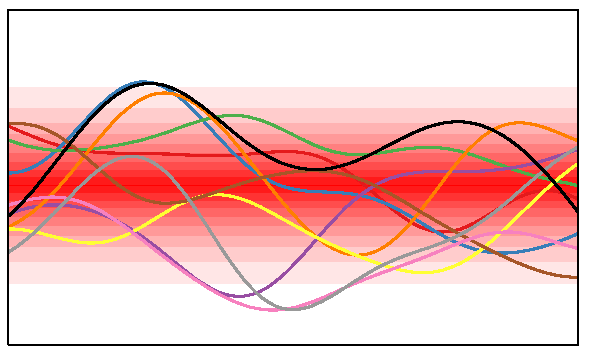
\includegraphics[width=0.48\textwidth]{\introfigsdir/fuzzy-0} & 
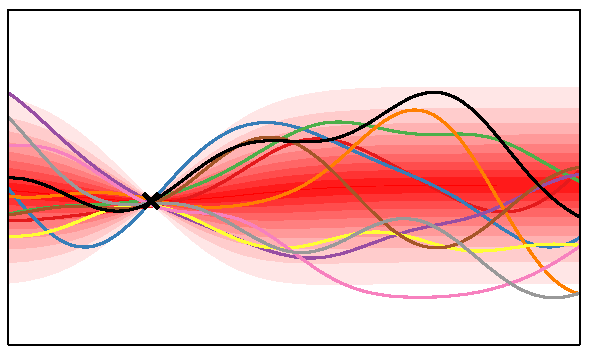
\includegraphics[width=0.48\textwidth]{\introfigsdir/fuzzy-1} \\
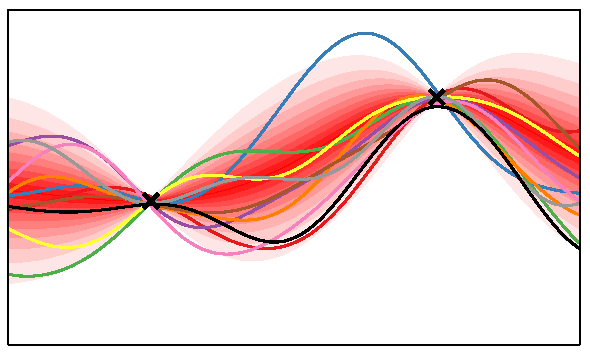
\includegraphics[width=0.48\textwidth]{\introfigsdir/fuzzy-2} & 
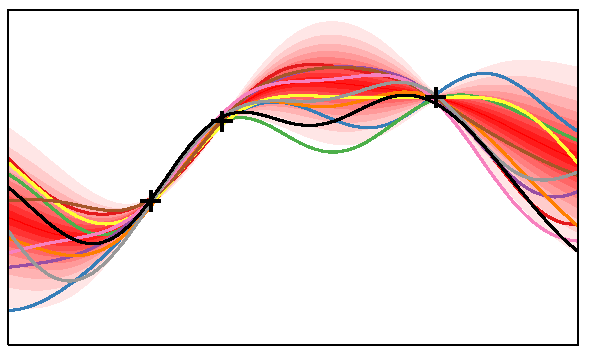
\includegraphics[width=0.48\textwidth]{\introfigsdir/fuzzy-3}
\end{tabular}
\end{centering}
\caption[One-dimensional Gaussian process posterior]{A visual representation of a one-dimensional Gaussian process posterior.
Shades of red show isocountours of the marginal density at each input location.
Coloured lines show samples from the process.
Top left: A \gp{} prior, not conditioned on any datapoints.
Other plots show the posterior as more
}
\label{fig:gp-post}
\end{figure}
%
%Figure \ref{fig:gp-post} shows a Gaussian process distribution, as it is conditioned on more and more observations.
%Typically, it's rendered with the mean and +- 2SD, but there's nothing special about mean.

Gaussian processes are distributions over functions such that any finite subset of function evaluations $f(x_1), f(x_2), \ldots f(x_N)$, have a joint Gaussian distribution \citep{rasmussen38gaussian}.
A \gp{} is completely specified by its mean function,
%
\begin{align}
%\mathbb{E}(f(x)) = \mu(x)
\expectargs{}{f(x)} = \mu(x)
\end{align}
%
and its covariance function, also called the \emph{kernel}:
%
\begin{align}
\Cov(f(x),f(x')) = \kernel(x,x')
\end{align}
%
It is common practice to assume zero mean, since marginalizing over an unknown mean function can be equivalently expressed as a zero-mean \gp{} with a new kernel.

The kinds of structure which can be captured by a \gp{} model is mainly determined by its kernel, which in turn determines how the model generalizes or extrapolates to new data.
One of the main difficulties in using \gp{}s lies in constructing a kernel which can represent the structure present in the data.
%  For small to medium-sized datasets, the kernel has a large impact on modeling efficacy.
%The structure of the kernel captures high-level properties of the unknown function, $f$, 
There are many possible choices of covariance function.
In fact, any symmetric positive-definite function can be used to construct a \gp{} model.
The benefit to this flexibility is that we can specify a wide range of models just by specifying the kernel.
%We can therefore define a language of regression models by specifying a language of kernels.

The class of models that could be called Gaussian processes is extremely broad.
Examples of commonly used models not usually cast as \gp{}s are linear regression, splines, some forms of generalized additive models, and Kalman filters.

Gaussian processes can be seen as a dual representation of Bayesian linear regression. \NA{Cite}
By moving into this dual space, we pay a price in computational complexity, but gain the ability to model functions to any desired level of detail.
Crucially, the marginal likelihood allows us to automatically discover the appropriate amount of detail to use, by Bayesian Occam's razor \citep{rasmussen2001occam,mackay2003information}.

For concreteness, we give the marginal likelihood of the data under a \gp{}:
%
\begin{align}
p(\vy | \vX, \mu(\cdot), k(\cdot, \cdot)) & = \N{\vy}{\mu(\vX)}{k(\vX, \vX)} \nonumber\\
& = (2\pi)^{-\frac{N}{2}}|k(\vX, \vX)|^{-\frac{1}{2}}\, \exp \left\{ -\frac{1}{2} \left( \vy - \boldsymbol\mu(\vX) \right)\tra k(\vX, \vX)\inv \left(\vy - \boldsymbol\mu(\vX) \right) \right\}
\label{eq:gp_marg_lik}
\end{align}
%
The Gaussian likelihood is referred to as the \emph{marginal} likelihood, since it implicitly integrates over all possible functions $\vy$.

Since the marginal likelihood depends on the kernel, we can select the form of the covariance function, or its parameters, by maximum likelihood, or through inference in a Bayesian model.

The predictive distributions also have a simple form:
%
\begin{align}
p( y(\iva^*) | \vy, \vX, \mu(\iva), k(\iva, \iva)) = \mathcal{N} \large( y(\iva^*) | & \mu(\iva^*) + k(\iva^*, \vX) k(\vX, \vX)\inv \left( \vy - \mu(\vX) \right)  \nonumber \\
& k(\iva^*, \iva^*) - k(\iva^*, \vX) k(\vX, \vX)\inv k(\vX, \iva^*) \large)
\label{eq:predictive}
\end{align}
%
These equations may look complex, but only require a few matrix operations to evaluate.

Sampling from a \gp{} is also straightforward: a sample from a \gp{} is just a single sample from a single multivariate Normal distribution \eqref{eq:predictive}.
Figure~\ref{fig:gp-post} shows prior and posterior samples from a \gp{}.


%[explain how that works]
% Insert neural net stuff here?

\subsection{Useful properties of Gaussian processes}

\begin{itemize}

\item {\bf Analytic inference}
Given a kernel function and some observations, the predictive posterior distribution can be computed exactly in closed form.  This is a rare property for nonparametric models to have.

\item {\bf Expressivity}
By choosing different covariance functions, we can express a very wide range of modeling assumptions.

\item {\bf Integration over hypotheses}
The fact that a \gp{} posterior lets us exactly integrate over a wide range of hypotheses means that overfitting is less of an issue than in comparable model classes.
It also removes the need for sophisticated optimization schemes.
%
In contrast, much of the neural network literature is devoted to techniques for regularization and optimization.

\item {\bf Marginal likelihood}
A side benefit of being able to integrate over all hyoptheses is that we compute the \emph{marginal likelihood} of the data given the model.
This gives us a principled way of comparing different Gaussian process models.

\item {\bf Closed-form posterior}
The posterior predictive distribution of a \gp{} is another \gp{}.
This means that \gp{}s can easily be composed with other models or decision procedures.
For example, in reinforcement learning applications, 

\item {\bf Easy to Analyze}
%\subsection{Why stick to such a limited model class?}
It may seem unsatisfying to restrict ourselves to a limited model class.
Shouldn't we instead learn to use some more flexible model class, such as the set of all computible functions?
The answer is: simple models can be used as well-understood building blocks for constructing more interesting models in diverse settings.

Consider linear models.
Although they form an extremely limited model class, they are fast, simple, and easy to analyze.
This makes them easy to incorporate into other models or procedures.
Linear models may seem like a hopelessly simple model class, but they're arguably the most useful modeling tools in existence.

\end{itemize}




\subsection{Limitations of Gaussian processes}

\begin{itemize}

\item {\bf Slow inference}
Computing the matrix inverse in \eqref{eq:gp_marg_lik} and \eqref{eq:predictive} takes $\mathcal{O}(N^3)$ time.
%and $\mathcal{O}(N^2)$ memory.  
Fortunately, this problem can be addressed by approximate inference schemes, and most \gp{} software packages implement several of these.

\item {\bf Light tails}
We may wish to use non-Gaussian noise models, for instance in order to be robust to outliers, or to perform classification, or some other form of structured prediction.
Using non-Gaussian noise models requires approximate inference schemes; fortunately, mature software packages exist which can automatically perform approximate inference for a wide variety of likelihoods.
%\item {\bf Symmetric}
%The predictive distribution of a \gp{} is always symmetric about its mean function.
%This means that \gp{} models are inappropriate for modeling non-negative functions, such as likelihoods.
%However, this problem can be addressed by simply exponentiating a \gp{} model, giving rise to a \emph{log-Gaussian process}.

\item {\bf The need to choose a kernel}
In practice, the extreme flexibility of \gp{} models means that we are also faced with the difficult task of choosing a kernel.
In fact, 
%because the model only depends on the inputs through the kernel, 
choosing a useful kernel is equivalent to the problem of learning good features for the data.
Typically, human experts choose from among a small set of standard kernels.
In this thesis, we hope to go some way towards automating the construction and selection of useful kernels.
\end{itemize}





\section{Outline and Contributions of this Thesis}

This thesis presents a set of related results about how the probabilistic nature of Gaussian process models allows them to be easily extended or composed with other models.
Furthermore, the fact that the marginal likelihood is often available (or easily approximable) means that we can evaluate how much evidence the data provides for one structure over another.

\paragraph{Chapter \ref{ch:kernels}} contains a wide-ranging overview of many of the types of structured priors on functions that can be easily expressed by constructing appropriate covariance functions.
%describes, in detail, the ways in which different sorts of structure can be introduced into a \gp{} model through the kernel.
%TODO: Expand this description.
For example, in chapter~\ref{ch:kernels}, we'll see how \gp{}s can be combined with latent variable models to produce models of nonparametric manifolds.
By introducing structure into the kernels of those \gp{}s, we can create manifolds with diverse topological structures, such as cylinders, torii and M\"obius strips.

Given a wide variety of structures, plus the ability to evaluate the suitability of each one, it's straightforward to automatically search over models.
{\bf Chapter \ref{ch:grammar}} shows how to construct a general, open-ended language over kernels - which implies a corresponding language over models.
In chapter~\ref{ch:grammar}, we'll see how the marginal likelihood can guide us into automatically building structured models, and how capturing structure allows us to extrapolate, rather than simply interpolating.

Another benefit of using a relatively simple model class is that the resulting models are easy to understand.
{\bf Chapter~\ref{ch:description}} demonstrates how easy-to-understand the resulting models are, by demonstrating a simple system which automatically describes the structure discovered in a dataset by a search over \gp{} models.
This system automatically generates reports with graphs and english-language descriptions of \gp{} models.
Chapter \ref{ch:description} shows that, for the particular language of models constructed in chapter \ref{ch:grammar}, it's relatively easy to automatically generate english-language descriptions of the models discovered.
Augmented with interpretable plots decomposing the predictive posterior, we demonstrate how to automatically generate useful analyses of time-series.
Combined with the automatic model search developed in chapter \ref{ch:grammar}, this system represents the beginnings of an ``automatic statistician''.
We discuss the advantages and potential pitfalls of automating the modeling process in this way.

{\bf Chapter \ref{ch:additive}} examines the model class obtained by performing dropout in \gp{}s, finding them to have equivalent covariance to \emph{additive Gaussian processes}, a model summing over exponentially-many \gp{} models, each depending on a different subset of the input variables.  An polynomial-time algorithm for doing inference in this model class is given, and the resulting model class is characterized and related to existing model classes.

{\bf Chapter \ref{ch:warped}} develops an extension of the \gplvm{} in which the latent distribution is a mixture of Gaussians.  This model gives rise to a Bayesian clustering model in the clusters have nonparametric shapes.  Like the density manifolds learned by the \gplvm{}, the shapes of the clusters learned by the \iwmm{} follow the contours of the data density.

Besides having a dual representation as linear regression, \gp{}s can also be derived as the limit of an infinitely-wide neural network.
As an example of using \gp{}s as a simple-to-understand building block, {\bf Chapter \ref{ch:deep-limits}} analyzes deep network models by characterizing the prior over functions obtained by composing \gp{} priors to form \emph{deep Gaussian processes}.
%, and relates them to existing neep neural network architecures.
We find that, as the number of layers in such models increases, the amount of information retained about the original input diminshes to a single degree of freedom.
We show that a simple change to the network architecture fixes this pathology.


\section{Attribution}

This thesis was made possible (and enjoyable to produce) by the substantial contributions of the many co-authors I was fortunate to work with.
In this section, I %detail the novel contributions of this thesis, and 
attempt to give proper credit to my tireless co-authors.

\paragraph{Structure through kernels}
%Chapter \ref{ch:kernels} contains a wide-ranging overview of many of the types of structured priors on functions that can be easily expressed by constructing appropriate covariance functions.
Section \ref{sec:deep_kernels} of chapter \ref{ch:kernels}, describing how symmetries in the kernel of a \gplvm{} give rise to priors on manifolds with interesting topologies, is based on a collaboration with David Reshef, Roger Grosse, Josh Tenenbaum, and Zoubin Ghahramani.

\paragraph{Structure Search}
The research upon which Chapter \ref{ch:grammar} is based was done in collaboration with James Robert Lloyd, Roger Grosse, Joshua B. Tenenbaum, and Zoubin Ghahramani, and was published in \citep{DuvLloGroetal13}, where James Lloyd was joint first author.
Myself, James Lloyd and Roger Grosse jointly developed the idea of searching through a grammar-based language of \gp{} models, inspired by \citet{grosse2012exploiting}, and wrote the first versions of the code together.
James Lloyd ran almost all of the experiments.
 Carl Rasmussen, Zoubin Ghahramani and Josh Tenenbaum provided many conceptual insights, as well as suggestions about how the resulting procedure could be most fruitfully applied.

\paragraph{Automatic Statistician} The work appearing in chapter \ref{ch:description} was written in collaboration with James Robert Lloyd, Roger Grosse, Joshua B. Tenenbaum, Zoubin Ghahramani, and was published in \citep{LloDuvGroetal14}.
The idea of the correspondence between kernels and adjectives grew out of discussions between James and myself.
James Lloyd wrote most of the code to automatically generate reports, and ran all of the experiments.
The text was written mainly by myself, James Lloyd, and Zoubin Ghahramani, with many helpful contributions and suggestions from Roger Grosse and Josh Tenenbaum.

\paragraph{Additive Gaussian processes}
The work in chapter \ref{ch:additive} discussing additive \gp{}s was done in collaboration with Hannes Nickisch and Carl Rasmussen, who developed a richly parameterized kernel which efficiently sums all possible products of input dimensions.
My role in the project was to examine the properties of the resulting model, clarify the connections to existing methods, and to create all figures and run all experiments.
This work was previously published in \citep{duvenaud2011additive11}.

\paragraph{Warped Mixtures}
The work comprising the bulk of chapter \ref{ch:warped} was done in collaboration with Tomoharu Iwata and Zoubin Ghahramani, and appeared in \citep{IwaDuvGha12}.
Specifically, the main idea was borne out of a conversation between Tomo and myself, and together we wrote almost all of the code together as well as the paper.
Tomo ran most of the experiments.
Zoubin Ghahramani provided initial guidance, as well as many helpful suggestions throughout the project.


\paragraph{Deep Gaussian Processes}
The ideas contained in chapter \ref{ch:deep-limits} were developed through discussions with Oren Rippel, Ryan Adams and Zoubin Ghahramani, and appear in \citep{DuvRipAdaGha14}.  The derivations, experiments and writing were done mainly by myself, with many helpful suggestions by my co-authors.

\outbpdocument{
\bibliographystyle{plainnat}
\bibliography{references.bib}
}


